\begin{figure}[htbp]

\begin{center}
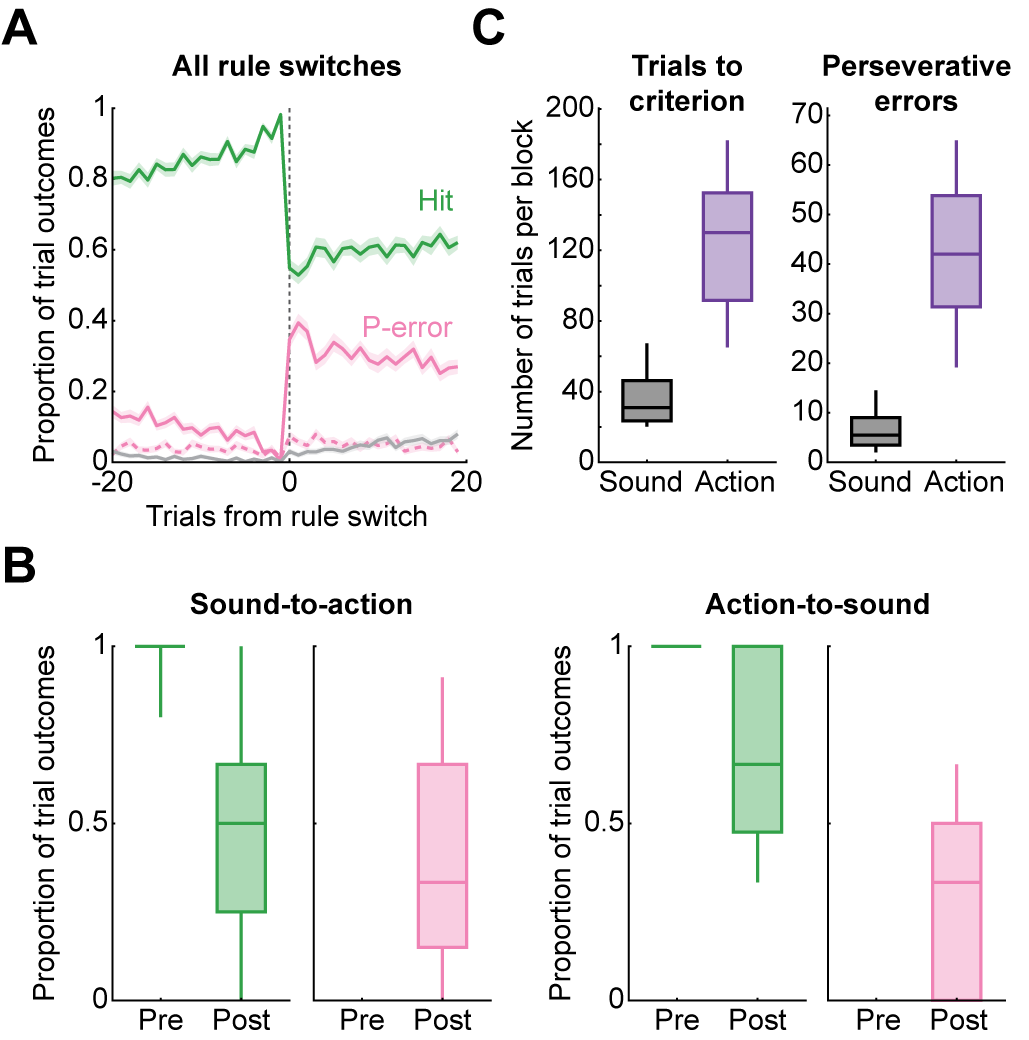
\includegraphics[width=8.7cm]{Figures/Fig3.png} 
\end{center}

\caption[Formal measures of task performance.]
{Formal measures of task performance. (A) Mean proportion of hits (green), perseverative errors (solid pink), other errors (dashed pink), and misses (gray) as a function of the number of trials from a rule switch across all sessions ($N=65$). Shading, SEM. (B) Boxplots representing the mean proportion of hits (green) and preseverative errors (pink) for trials immediately preceding a rule switch (Pre) and for trials immediately following one (Post). Results are presented separately for switches from the sound rule to an action rule (left), and vice-versa (right). (C) Boxplots representing the number of trials taken to reach criterion (left), and the number of perseverative errors committed (right), during sound (black) and action blocks (purple). All boxes indicate quartiles 1--3; whiskers indicate 9th and 91st percentiles.}

\label{fig:Fig3}
\end{figure}